\documentclass[twocolumn, letterpaper]{scrartcl}

\usepackage{uog_factsheet}
\usepackage{xcolor}
\usepackage{hyperref}

\definecolor{seablue}{RGB}{0,127,169}

\begin{document}
    \title{\color{seablue}User Consent \& Privacy Policies Project}

	\maketitle
	
    % \section*{Instructions}
    
    % \begin{itemize}
    %     \item Open history of your browser, choose 3 websites from your browsing history, open these 3 website in a private/incognito window
    %     \item Is there a consent banner? Does it comply with elements of valid consent (Free, specific, informed, unambiguous)?
    %     \item Check the slides to validate your analysis, write a 2-page report with your analysis.
    % \end{itemize}
    
    \section*{Website Choices}
        
         For the sake of diversity of industries, three websites were selected: \textbf{Games Workshop}\cite{GW} (the world's largest miniatures game retailer, see Fig. \ref{fig:a}), \textbf{Le Monde}\cite{LM} (A French newspaper, see Fig. \ref{fig:c}) and \textbf{LinkedIn}\cite{LD} (the largest professional social media, see Fig. \ref{fig:d}).
	
	\section{Analyses of the websites' policies and consent-handling}
	
	    We recall that consent forms are a mechanism to give data subjects control and choice over whether or not their personal data will be processed. It must be given before any processing starts and is only valid when four elements of valid consent (based on the General Data Protection Regulation's article 4(11)) are met: i) \textbf{Free}, ii) \textbf{Specific}, iii) \textbf{Informed}, iv) \textbf{Unambiguous}.
	
    \subsection*{Games Workshop's}

	    Games Workshop's cookie policy provides an \textbf{example of a policy that is neither free, specific, informed or unambiguous}.
	
    	\textbf{The consent policy is not free}. The data subjects have no choice when presented with the consent banner. It is more of a warning than a prompt: "\textit{This website uses cookies to personalise content and advertising, and to analyse our traffic. By continuing to use this site you are agreeing to our use of cookies}". We could qualify this instance as an \textit{imbalance of power} as coercion is involved -- the data subjects have no choice but to click on the \textit{continue} button. We also see here an example of \textit{conditionality} and \textit{detrimentality} (See Fig. \ref{fig:b}). To opt-out, the data subjects must personally set up their browsers to restrict cookies\footnote{Games Workshop does not provides ways to restrict the use of cookies. Instead, they explicitly mention that the data subjects should personally parameter their browser via the use of third-parties plug-ins or opt out of systems such as Google AdSense.}, they will experience a loss in website functionality. Finally, the right to withdraw consent (as per GDPR Article 7(3)) does not exist.
    	
    	\textbf{The consent policy is not specific}. The stated purpose of data usage is \textit{too wide}, mentioning cookies would be used "to personalise content and advertising, and to analyse our traffic" in the main page banner. Some detail is provided in their Cookie Notice page\cite{GW_CN} but the descriptions are not extensive (e.g. there is no indication how long any data is kept). A \textit{lack of granularity in consent requests is found there}, confirming the lack of choice exposed in the first paragraph.
    	
    	Given what we saw above, \textbf{the consent policy does not allow informed consent}. The language and instructions for people to opt out of tracking are not meant for lay people as shown in Footnote 1. Similarly, \textbf{the consent banner presents an example of ambiguous consent}. The only possible action is to "continue" and close the cookie banner.
    	
    	To sum up, Games Workshop has a lackluster implementation of a user consent and privacy policy in the context of GDPR. The company fails to meet all four criteria of a valid consent. Of note, the Cookie Notice page mentions that the website uses a technology called \textit{Web Beacon}, which is not fully stated in the main page's consent bar and which also cannot be opted-out.
 	
 		\begin{figure}
    % 		Figure 1\label{fig:a}. Games Workshop's Main Page
    		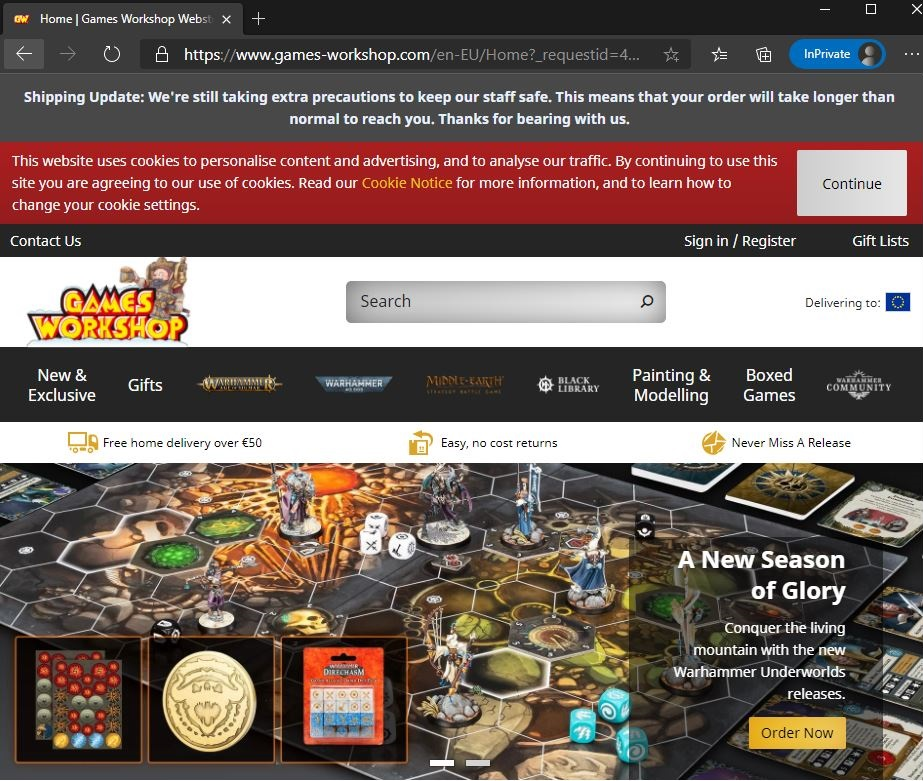
\includegraphics[width=0.95\linewidth]{gw_website.JPG}
     		\caption{Games Workshop's Main Page \label{fig:a}}
     	\end{figure}
    
        \begin{figure}[tbp]	
            % Figure 2\label{fig:b}. Example of conditionality in Games Workshop's policy
            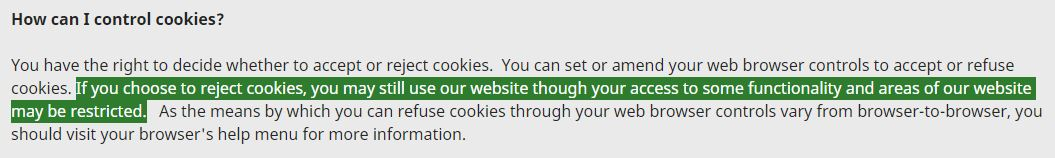
\includegraphics[width=0.95\linewidth]{conditionality.JPG}
            \caption{Example of conditionality in Games Workshop's policy \label{fig:b}}
        \end{figure}
        
	\subsection*{Le Monde's}

    	Le Monde's website provides elements that favors the interpretation that data subjects' consent is \textbf{free}, \textbf{specific}, \textbf{informed}, and \textbf{unambiguous}. However, we will present two caveats to this. 
        
    	Overall, there is no apparent of imbalance of power, conditionality or detrimentality, implying that consent can be freely given (e.g. Consent is asked in the scope of providing news content to the data subjects). Specificity is present as the purpose of collecting data is clearly stated and data subjects can opt-in to cookie tracking at a granular level. All the same, tracking options are ticked off by default in the cookie parameter page. The possibility to refuse all cookies, besides those legally-allowed to be non-opt-out, is available as well (Ssee Fig. \ref{fig:d}). Finally, consent seems to be informed as the purposes of data usage is stated on the front page (See Fig. \ref{fig:c}) and an exhaustive description of the collected data is detailed in the parameter page. There is no apparent ambiguity.
    	
    	\begin{figure}[tbp]	
            % Figure 3\label{fig:c}. Le Monde's Main Page 
            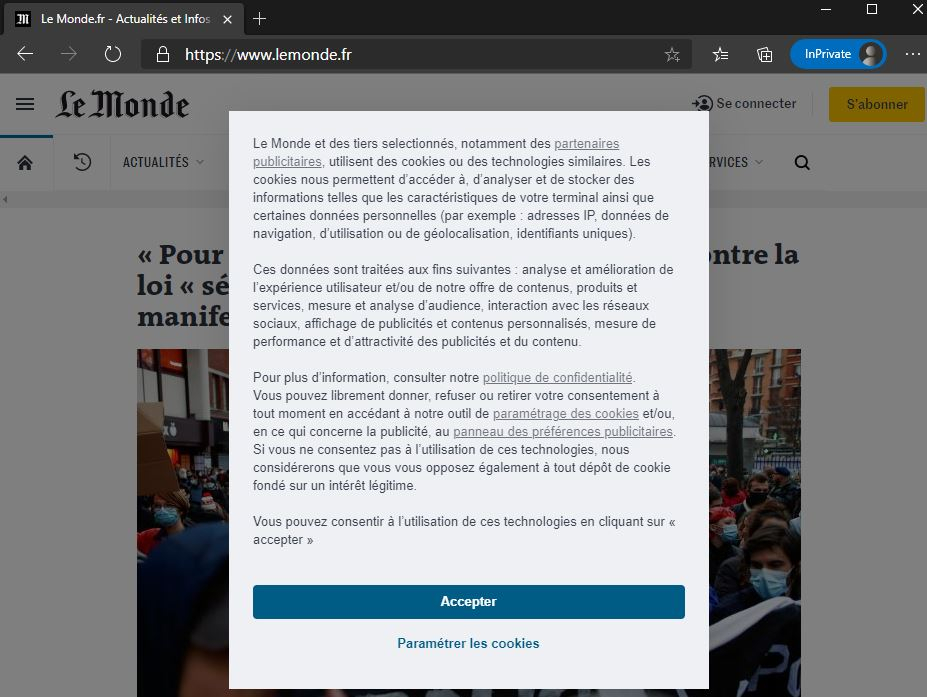
\includegraphics[width=0.9\linewidth]{lm_website.JPG}
            \caption{Le Monde's Main Page \label{fig:c}}
        \end{figure}
        
    	However, the validity of the data subjects' consent can be put into question as, were they to refuse all cookies, Le Monde's website would constantly display a irremovable ad (for their subscription service) that is obstructing on some devices (See Fig. \ref{fig:e}). \textbf{This could unmake the argument that Le Monde's policy fulfills the 'free' criterion of valid consent as stated by Article 4(11) of GDPR}. This irremovable ad could be considered a detriment and a consequence of not consenting. On the other hand, \textit{there is no prior indication that this bar would appear if the cookies were deactivated}. This bar is not used as a threat to the data subjects' user experience. In the end, it might only be an issue on some devices for which the website was not optimized for. 
    	
    	\begin{figure}[tbp]
            % Figure 4\label{fig:d}. Le Monde's Cookie Policy Parameter Page 
            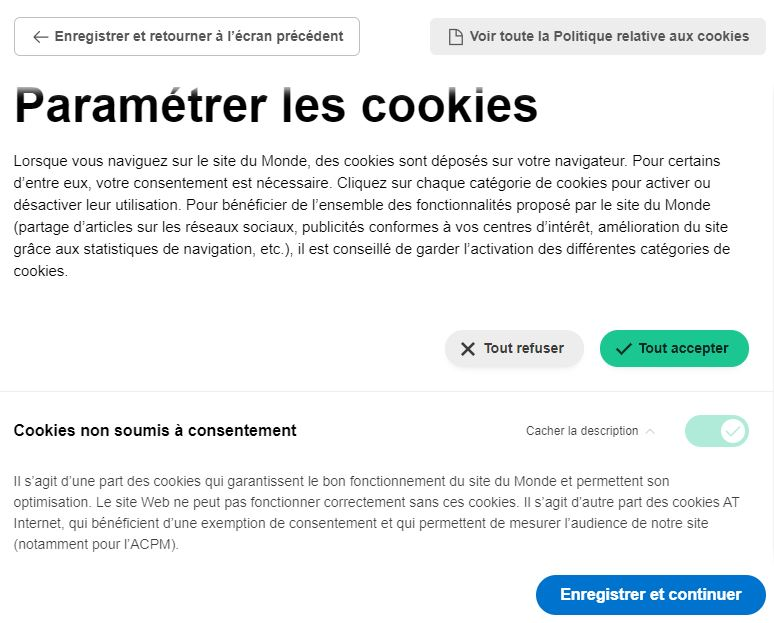
\includegraphics[width=0.9\linewidth]{lm_cn.JPG}
            \caption{Le Monde's Cookie Policy Parameter Page \label{fig:d}}
        \end{figure}
        
    	Another weak point relates to accessing Le Monde's Cookies and Privacy Policy page\cite{LM2}. It happens to be \textbf{unreadable if the data subjects have not yet accepted the policy}, i.e. there is no way for data subjects to read the detailed policy (which includes a table detailing the cookies used by Le Monde, the collected and shared data, and an assiociated purpose and expiration date) without accepting the cookies first (See Fig. \ref{fig:f}). This implies that there might not be an informed consent on Le Monde's website and Recital\$42 and Article 7(3) of GDPR might not be fully satisfied. 
        
        \begin{figure}[tbp]
            % Figure 5\label{fig:e}. Le Monde's Unremovable Ad Bar
            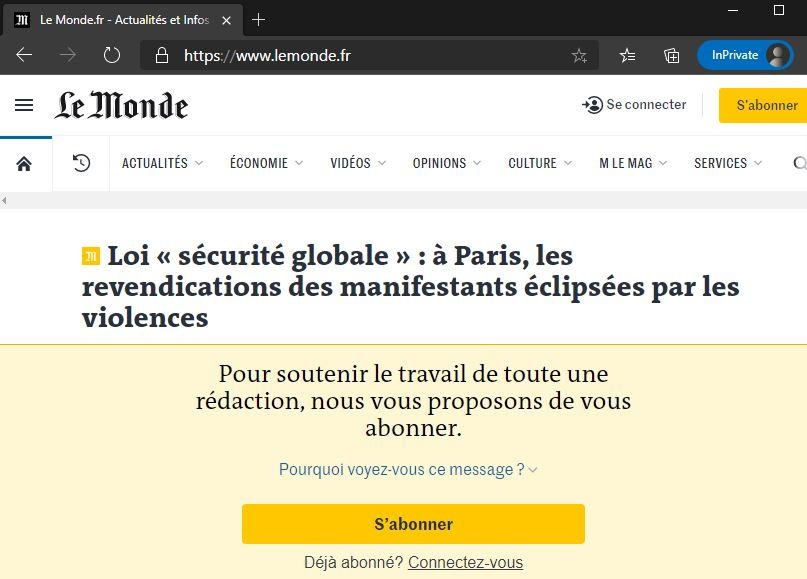
\includegraphics[width=0.95\linewidth]{lm_sub.JPG}
            \caption{Le Monde's Unremovable Ad \label{fig:e}}
        \end{figure}
        
        \begin{figure}[tbp]	
            % Figure 6\label{fig:f}. Le Monde's Unreadable Detailed Cookie Policy
            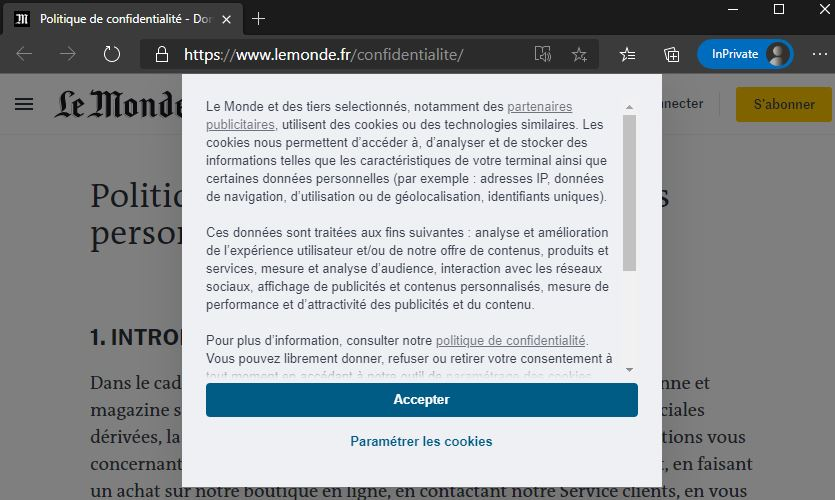
\includegraphics[width=0.95\linewidth]{lm_policy.JPG}
            \caption{Le Monde's Unreadable Detailed Cookie Policy\label{fig:f}}
        \end{figure}
        
        \begin{figure}[tbp]	
        % Figure 6\label{fig:g}. LinkedIn's Main Page 
        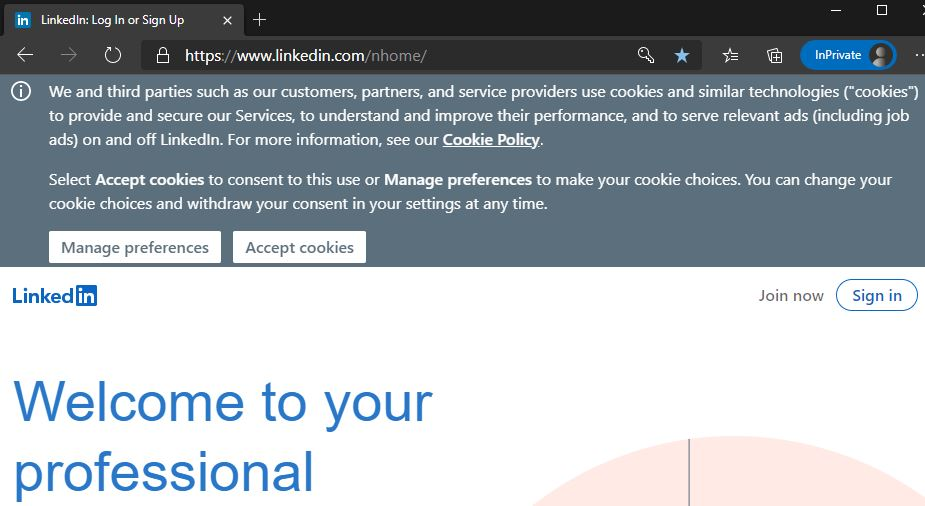
\includegraphics[width=0.95\linewidth]{ld_website.JPG}
        \caption{LinkedIn's Main Page \label{fig:g}}
        \end{figure}
        
	\subsection*{LinkedIn's}
	    
	    Similar to Le Monde's website, LinkedIn provides elements proving that consent given by data subjects is \textbf{free}, \textbf{specific}, \textbf{informed}, and \textbf{unambiguous}. For instance, LinkedIn provides a detailed consent bar (See Fig. \ref{fig:g}) as well as a dedicated cookie page where data subjects can decide to opt-in (See Fig. \ref{fig:h}).
        
	    As with Le Monde, LinkedIn does provide a detailed Cookie Policy page that contains a table dedicated to describing the type of cookies used, the data collected and shared, and an associated purpose and expiration date (LinkedIn does \textit{hide} that page behind a pop-up).
	    
	    LinkedIn's weak point is that, were the data subjects leaving the cookie policy parameter page without inputing any modification (See Fig. \ref{fig:h}), the consent bar would never appear again. I.e. Once the cookie parameters have been opened, the website considers them modified and accepted by the data subjects. Afterward, finding the parameter page again is complex. This implies \textbf{withdrawal of consent} can be hard to perform.

        \begin{figure}[tbp]	
        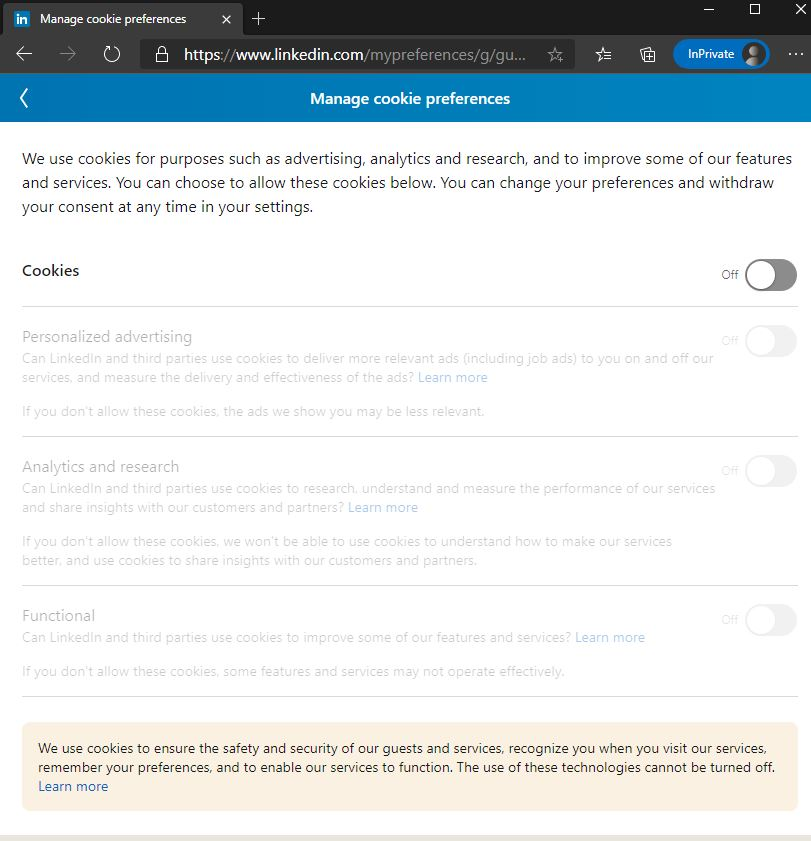
\includegraphics[width=0.9\linewidth]{ld_cn.JPG}
        \caption{LinkedIn's Cookie Policy Parameter Page \label{fig:h}}
        \end{figure}
        
        \begin{figure}[tbp]	
        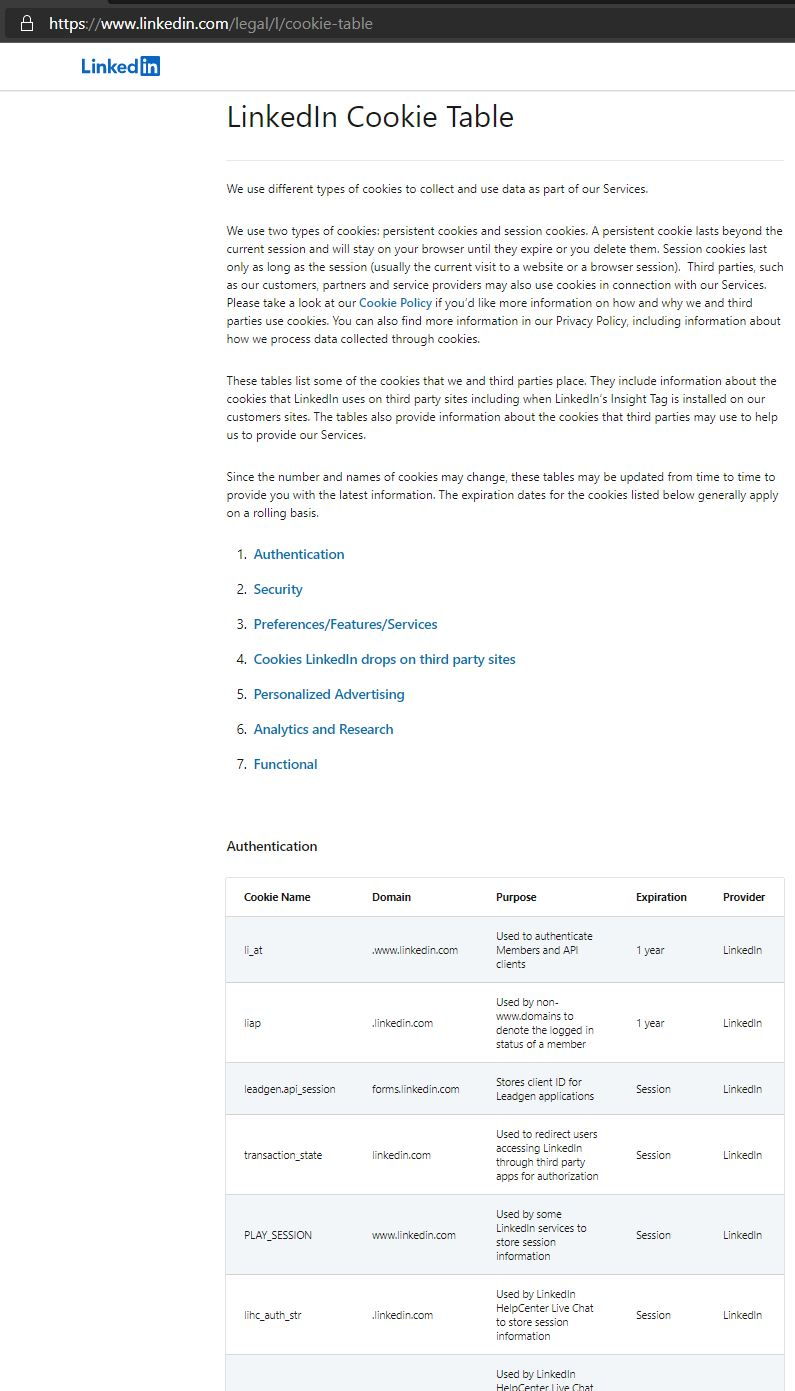
\includegraphics[width=0.9\linewidth]{ld_table.JPG}
        \caption{LinkedIn's Cookie Detailed Policy Page \label{fig:i}}
        \end{figure}
        
	\subsection*{Conclusion}
	
	Out of all three websites, Games Workshop's is the most at fault in how it handles consent. It fails in all four validity categories set by the Article 4(11) of GDPR.
	
	Le Monde and LinkedIn's websites are much more compliant with the article, scoring in all four categories. However, both websites shows failings in some cases, meaning that doubts can still be cast on the validity of consent on their platforms.
	
    \bibliographystyle{unsrtnat}   
    \begin{thebibliography}{9}

    \bibitem{GW}
    	Games Workshop Limited, \textit{\href{https://www.games-workshop.com/en-US/Home}{website}}.
    \bibitem{LM}
    	Le Monde SA, \textit{\href{https://www.lemonde.fr/}{website}}.
    \bibitem{LD}
    	LinkedIn Corporation, \textit{\href{https://www.linkedin.com/}{website}}.
    \bibitem{GW_CN}
    	Games Workshop's Cookie Notice page, \textit{\href{https://www.games-workshop.com/en-EU/Cookie-Notice}{website}}.
    \bibitem{LM2}
    	Le Monde's Detailed Cookies and Privacy Page, \textit{\href{https://www.lemonde.fr/confidentialite/}{website}}.

    \end{thebibliography}

\end{document}

